\def\pgfsysdriver{pgfsys-dvisvgm.def}
% flashcards-title: Local interaction rules producing a group pattern
% flashcards-desc: In the first panel organism dots have scattered movement arrows. In the later panel they are close together with aligned arrows.
\documentclass[tikz,border=6pt]{standalone}
\usetikzlibrary{arrows.meta,calc,fit,positioning,shapes.geometric}

\definecolor{fcink}{HTML}{17212B}
\definecolor{fcblue}{HTML}{1D5D8C}
\definecolor{fcgreen}{HTML}{2D6A4F}
\definecolor{fcorange}{HTML}{A44A1F}
\definecolor{fcpale}{HTML}{F4F7F9}
\definecolor{fcsoil}{HTML}{8B5E3C}

\tikzset{
  fc text/.style={font=\sffamily, text=fcink},
  fc panel/.style={draw=fcink, line width=0.9pt, rounded corners=5pt, fill=fcpale},
  fc node/.style={draw=fcink, line width=0.9pt, rounded corners=4pt, fill=white,
    minimum width=24mm, minimum height=10mm, align=center, font=\sffamily},
  fc arrow/.style={-{Stealth[length=3.2mm,width=2.4mm]}, line width=1.2pt,
    draw=fcblue, line cap=butt},
  fc boundary/.style={draw=fcorange, line width=1.4pt, dash pattern=on 5pt off 3pt,
    rounded corners=7pt},
  fc label/.style={font=\sffamily\bfseries, text=fcink},
  fc note/.style={font=\sffamily\small, text=fcink, align=center}
}

\begin{document}
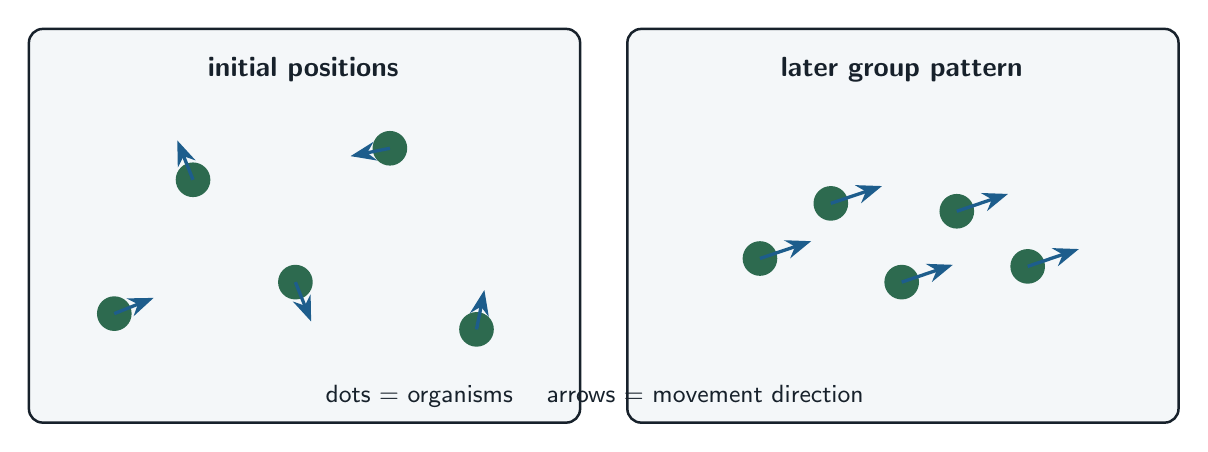
\begin{tikzpicture}[fc text, x=1cm, y=1cm]
  \node[fc panel, minimum width=70mm, minimum height=50mm, anchor=south west] at (0,0) {};
  \node[fc panel, minimum width=70mm, minimum height=50mm, anchor=south west] at (7.6,0) {};
  \node[fc label] at (3.5,4.5) {initial positions};
  \node[fc label] at (11.1,4.5) {later group pattern};
  \foreach \x/\y/\dx/\dy in {1.1/1.4/.5/.2,2.1/3.1/-.2/.5,3.4/1.8/.2/-.5,4.6/3.5/-.5/-.1,5.7/1.2/.1/.5} {
    \fill[fcgreen] (\x,\y) circle (2.2mm); \draw[fc arrow] (\x,\y)--+(\dx,\dy);
  }
  \foreach \x/\y in {9.3/2.1,10.2/2.8,11.1/1.8,11.8/2.7,12.7/2.0} {
    \fill[fcgreen] (\x,\y) circle (2.2mm); \draw[fc arrow] (\x,\y)--+(.65,.22);
  }
  \node[fc note] at (7.2,0.35) {dots = organisms \quad arrows = movement direction};
\end{tikzpicture}
\end{document}
